\documentclass{beamer}
\title{向量与线性运算}
\begin{document}

\begin{frame}{什么是向量？}
我们熟悉的速度、位移和力，都既有大小，又有方向。
\begin{definition}[几何向量]
具有\blue{大小}和\blue{方向}的量称为向量。
记作 $\vec v=(x,y)\in\bF^2$。
\end{definition}
\pp
\begin{example}
从原点指向点 $(2,1)$ 的向量为
\[\vec v=\begin{pmatrix}2\\1\end{pmatrix}.\]
\end{example}
\end{frame}

\begin{frame}{向量加法}
\begin{theorem}[交换律]
对任意向量 $\vec u,\vec v$，有
\[\vec u+\vec v=\vec v+\vec u.\]
\end{theorem}
\pause
\begin{proof}
由平行四边形法则，两种顺序得到同一条对角线。
\end{proof}
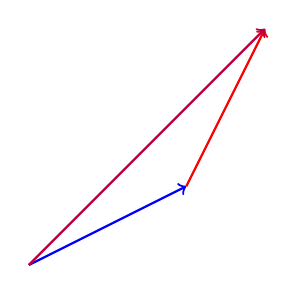
\begin{tikzpicture}
\draw[->,thick,blue] (0,0)--(2,1);
\draw[->,thick,red] (2,1)--(3,3);
\draw[->,thick,purple] (0,0)--(3,3);
\end{tikzpicture}
\end{frame}

\begin{frame}{自定义符号与待处理内容}
递归宏：$\mEnd(\mU)$；算子：$\rank A$。
\begin{observation}
导入样式文件后，自定义数学环境也能统一排版。
\end{observation}
\only<2->{这段 overlay 内容默认显示。}
\mysterycommand{未知内容会原样保留，并出现在警告列表。}
\xymatrix{U \ar[r]^f & V}
\end{frame}
\end{document}
